% Options for packages loaded elsewhere
\PassOptionsToPackage{unicode}{hyperref}
\PassOptionsToPackage{hyphens}{url}
%
\documentclass[
]{article}
\usepackage{amsmath,amssymb}
\usepackage{iftex}
\ifPDFTeX
  \usepackage[T1]{fontenc}
  \usepackage[utf8]{inputenc}
  \usepackage{textcomp} % provide euro and other symbols
\else % if luatex or xetex
  \usepackage{unicode-math} % this also loads fontspec
  \defaultfontfeatures{Scale=MatchLowercase}
  \defaultfontfeatures[\rmfamily]{Ligatures=TeX,Scale=1}
\fi
\usepackage{lmodern}
\ifPDFTeX\else
  % xetex/luatex font selection
\fi
% Use upquote if available, for straight quotes in verbatim environments
\IfFileExists{upquote.sty}{\usepackage{upquote}}{}
\IfFileExists{microtype.sty}{% use microtype if available
  \usepackage[]{microtype}
  \UseMicrotypeSet[protrusion]{basicmath} % disable protrusion for tt fonts
}{}
\makeatletter
\@ifundefined{KOMAClassName}{% if non-KOMA class
  \IfFileExists{parskip.sty}{%
    \usepackage{parskip}
  }{% else
    \setlength{\parindent}{0pt}
    \setlength{\parskip}{6pt plus 2pt minus 1pt}}
}{% if KOMA class
  \KOMAoptions{parskip=half}}
\makeatother
\usepackage{xcolor}
\usepackage[margin=1in]{geometry}
\usepackage{longtable,booktabs,array}
\usepackage{calc} % for calculating minipage widths
% Correct order of tables after \paragraph or \subparagraph
\usepackage{etoolbox}
\makeatletter
\patchcmd\longtable{\par}{\if@noskipsec\mbox{}\fi\par}{}{}
\makeatother
% Allow footnotes in longtable head/foot
\IfFileExists{footnotehyper.sty}{\usepackage{footnotehyper}}{\usepackage{footnote}}
\makesavenoteenv{longtable}
\usepackage{graphicx}
\makeatletter
\def\maxwidth{\ifdim\Gin@nat@width>\linewidth\linewidth\else\Gin@nat@width\fi}
\def\maxheight{\ifdim\Gin@nat@height>\textheight\textheight\else\Gin@nat@height\fi}
\makeatother
% Scale images if necessary, so that they will not overflow the page
% margins by default, and it is still possible to overwrite the defaults
% using explicit options in \includegraphics[width, height, ...]{}
\setkeys{Gin}{width=\maxwidth,height=\maxheight,keepaspectratio}
% Set default figure placement to htbp
\makeatletter
\def\fps@figure{htbp}
\makeatother
\setlength{\emergencystretch}{3em} % prevent overfull lines
\providecommand{\tightlist}{%
  \setlength{\itemsep}{0pt}\setlength{\parskip}{0pt}}
\setcounter{secnumdepth}{5}
\usepackage{booktabs}
\usepackage{longtable}
\usepackage{array}
\usepackage{multirow}
\usepackage{wrapfig}
\usepackage{float}
\usepackage{colortbl}
\usepackage{pdflscape}
\usepackage{tabu}
\usepackage{threeparttable}
\usepackage{threeparttablex}
\usepackage[normalem]{ulem}
\usepackage{makecell}
\usepackage{xcolor}
\ifLuaTeX
  \usepackage{selnolig}  % disable illegal ligatures
\fi
\usepackage{bookmark}
\IfFileExists{xurl.sty}{\usepackage{xurl}}{} % add URL line breaks if available
\urlstyle{same}
\hypersetup{
  pdftitle={Predicting GPA and Interpreting Results},
  pdfauthor={Brandon Chan, Lucas Duncan, Owen Macgowan},
  hidelinks,
  pdfcreator={LaTeX via pandoc}}

\title{Predicting GPA and Interpreting Results}
\author{Brandon Chan, Lucas Duncan, Owen Macgowan}
\date{2025-03-07}

\begin{document}
\maketitle

{
\setcounter{tocdepth}{2}
\tableofcontents
}
\section{Executive Summary and
Contents}\label{executive-summary-and-contents}

\begin{longtable}[]{@{}
  >{\raggedleft\arraybackslash}p{(\columnwidth - 4\tabcolsep) * \real{0.0667}}
  >{\raggedright\arraybackslash}p{(\columnwidth - 4\tabcolsep) * \real{0.4111}}
  >{\raggedright\arraybackslash}p{(\columnwidth - 4\tabcolsep) * \real{0.5222}}@{}}
\toprule\noalign{}
\begin{minipage}[b]{\linewidth}\raggedleft
Index
\end{minipage} & \begin{minipage}[b]{\linewidth}\raggedright
Category
\end{minipage} & \begin{minipage}[b]{\linewidth}\raggedright
Method
\end{minipage} \\
\midrule\noalign{}
\endhead
\bottomrule\noalign{}
\endlastfoot
1 & Introduction and Tidying & Importing, Wrangling and Encoding \\
2 & Unsupervised Learning and Analysis & PCA and Clustering \\
3 & Preprocessing & Variable Selection \\
4 & Supervised Regression & Linear and Non-Linear Regression \\
5 & Supervised Linear Classification & LDA and Logistic Regression \\
6 & Supervised Non-Linear Classification & Tree-Based Methods and
Support Vector Machines \\
7 & Deep Learning & Neural Network \\
8 & Conclusion and Future Research & Written Description \\
\end{longtable}

\section{Introduction and
Preprocessing}\label{introduction-and-preprocessing}

By analyzing different factors that contribute to student performance,
we aim to provide insight into how institutions can improve educational
and environmental factors that foster student success. This is an issue
that we can relate to directly. As students ourselves, we understand
that success in academics is influenced by several factors that include
preparation and ability, but go beyond to include factors outside of
school.

\subsection{The Student Performance
Dataset}\label{the-student-performance-dataset}

The dataset consists of attributes that may have an impact on
performance in school. There are academic variables that include grades
in different subjects and other variables like ethnicity, gender, and
economic status of the student families. There are options for
regression and classification problems with this data. With the given
variables, GPA seems like the most likely response variable to represent
student performance. After some wrangling, gpa\_letter, gpa, and
gpa\_desirable represent different forms of the possible response
variable to predict.

We start by cleaning our data; renaming columns for clarity, converting
column types, generating attributes, and filtering rows and columns. We
filter duplicate rows, and interpolate using column means for missing
numerical variables, we fill variables where possible to fix
inconsistencies between gpa and gpa\_letter, then drop the remaining
rows missing key factor variables.

\begin{longtable}[]{@{}
  >{\raggedleft\arraybackslash}p{(\columnwidth - 20\tabcolsep) * \real{0.0488}}
  >{\raggedright\arraybackslash}p{(\columnwidth - 20\tabcolsep) * \real{0.0915}}
  >{\raggedright\arraybackslash}p{(\columnwidth - 20\tabcolsep) * \real{0.1037}}
  >{\raggedleft\arraybackslash}p{(\columnwidth - 20\tabcolsep) * \real{0.1280}}
  >{\raggedleft\arraybackslash}p{(\columnwidth - 20\tabcolsep) * \real{0.0793}}
  >{\raggedleft\arraybackslash}p{(\columnwidth - 20\tabcolsep) * \real{0.1098}}
  >{\raggedleft\arraybackslash}p{(\columnwidth - 20\tabcolsep) * \real{0.1280}}
  >{\raggedleft\arraybackslash}p{(\columnwidth - 20\tabcolsep) * \real{0.1280}}
  >{\raggedright\arraybackslash}p{(\columnwidth - 20\tabcolsep) * \real{0.0671}}
  >{\raggedleft\arraybackslash}p{(\columnwidth - 20\tabcolsep) * \real{0.0305}}
  >{\raggedright\arraybackslash}p{(\columnwidth - 20\tabcolsep) * \real{0.0854}}@{}}
\toprule\noalign{}
\begin{minipage}[b]{\linewidth}\raggedleft
is\_male
\end{minipage} & \begin{minipage}[b]{\linewidth}\raggedright
race\_ethnicity
\end{minipage} & \begin{minipage}[b]{\linewidth}\raggedright
parent\_education
\end{minipage} & \begin{minipage}[b]{\linewidth}\raggedleft
has\_subsidized\_lunch
\end{minipage} & \begin{minipage}[b]{\linewidth}\raggedleft
has\_prepared
\end{minipage} & \begin{minipage}[b]{\linewidth}\raggedleft
recent\_math\_score
\end{minipage} & \begin{minipage}[b]{\linewidth}\raggedleft
recent\_writing\_score
\end{minipage} & \begin{minipage}[b]{\linewidth}\raggedleft
recent\_science\_score
\end{minipage} & \begin{minipage}[b]{\linewidth}\raggedright
gpa\_letter
\end{minipage} & \begin{minipage}[b]{\linewidth}\raggedleft
gpa
\end{minipage} & \begin{minipage}[b]{\linewidth}\raggedright
gpa\_desirable
\end{minipage} \\
\midrule\noalign{}
\endhead
\bottomrule\noalign{}
\endlastfoot
1 & D & some college & 1 & 1 & 89 & 85 & 26 & C & 59.5 & TRUE \\
1 & B & high school & 1 & 0 & 65 & 67 & 96 & A & 82.0 & FALSE \\
\end{longtable}

\subsection{Variable Distributions}\label{variable-distributions}

We now want to get more familiar with our data, looking first at the
numeric columns, we observe all seem approximately normal, which is to
be expected given their nature. We note they all seem to be within
acceptable range (0,100). We next analyze the boolean columns, none of
which have one boolean option which dominated the data. Notably there
seems to be an approximately equal number of males and females, which is
a good sign that our sample is proportional to an entire group. Finally
we analyze the true factors, education and race, and once again no one
factor dominates the data, while factors are not exactly normally
distributed, nor should they be, there is healthy variation between rows
with no one factor representing too few rows.

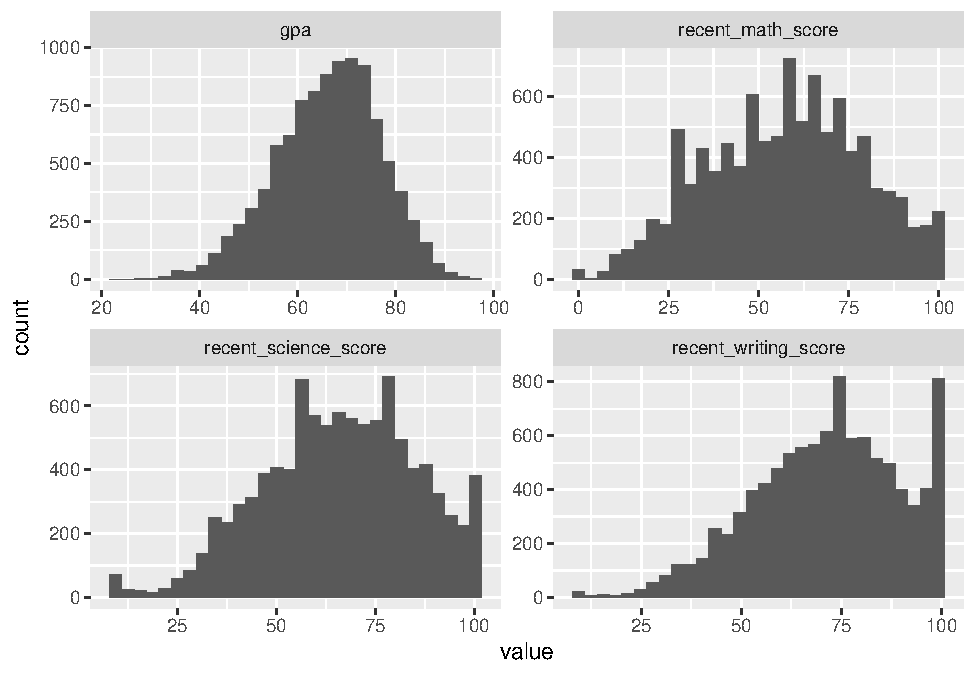
\includegraphics{ST494_FP_files/figure-latex/unnamed-chunk-5-1.pdf}
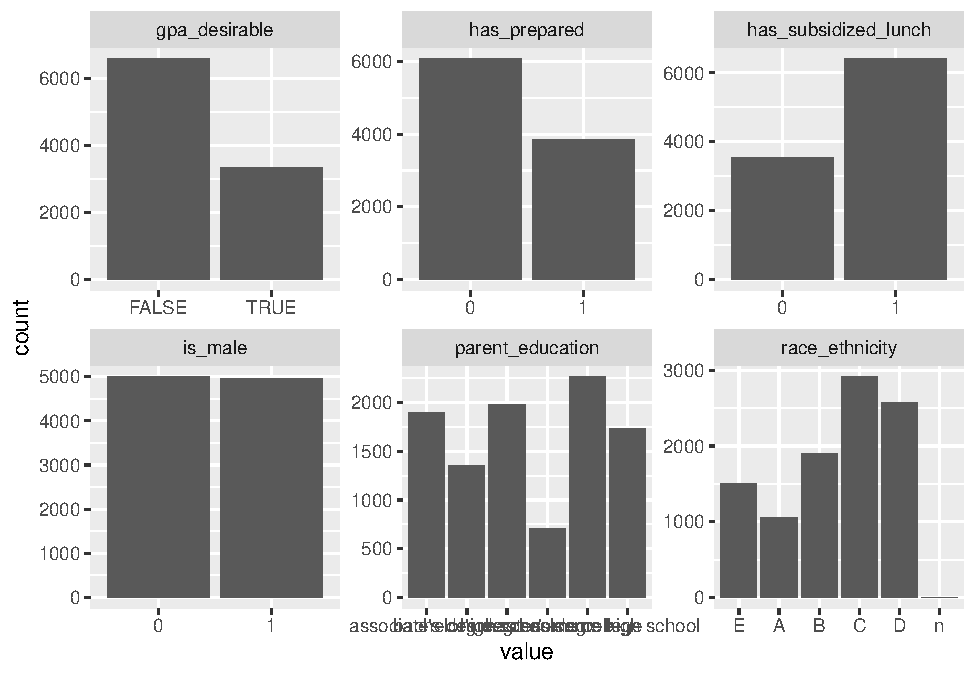
\includegraphics{ST494_FP_files/figure-latex/unnamed-chunk-5-2.pdf}

\subsection{Encoded Data Frame}\label{encoded-data-frame}

From here, our next step in processing is to convert our factor
variables into one hot notation to be used in predictive models. We
modify both parent\_education and race, as well as converting boolean
factor variables into integers for use in models.

\begin{longtable}[]{@{}
  >{\raggedleft\arraybackslash}p{(\columnwidth - 38\tabcolsep) * \real{0.0208}}
  >{\raggedleft\arraybackslash}p{(\columnwidth - 38\tabcolsep) * \real{0.0547}}
  >{\raggedleft\arraybackslash}p{(\columnwidth - 38\tabcolsep) * \real{0.0339}}
  >{\raggedleft\arraybackslash}p{(\columnwidth - 38\tabcolsep) * \real{0.0469}}
  >{\raggedleft\arraybackslash}p{(\columnwidth - 38\tabcolsep) * \real{0.0547}}
  >{\raggedleft\arraybackslash}p{(\columnwidth - 38\tabcolsep) * \real{0.0547}}
  >{\raggedright\arraybackslash}p{(\columnwidth - 38\tabcolsep) * \real{0.0286}}
  >{\raggedleft\arraybackslash}p{(\columnwidth - 38\tabcolsep) * \real{0.0130}}
  >{\raggedright\arraybackslash}p{(\columnwidth - 38\tabcolsep) * \real{0.0365}}
  >{\raggedleft\arraybackslash}p{(\columnwidth - 38\tabcolsep) * \real{0.0417}}
  >{\raggedleft\arraybackslash}p{(\columnwidth - 38\tabcolsep) * \real{0.0417}}
  >{\raggedleft\arraybackslash}p{(\columnwidth - 38\tabcolsep) * \real{0.0417}}
  >{\raggedleft\arraybackslash}p{(\columnwidth - 38\tabcolsep) * \real{0.0417}}
  >{\raggedleft\arraybackslash}p{(\columnwidth - 38\tabcolsep) * \real{0.0417}}
  >{\raggedleft\arraybackslash}p{(\columnwidth - 38\tabcolsep) * \real{0.0417}}
  >{\raggedleft\arraybackslash}p{(\columnwidth - 38\tabcolsep) * \real{0.0885}}
  >{\raggedleft\arraybackslash}p{(\columnwidth - 38\tabcolsep) * \real{0.0729}}
  >{\raggedleft\arraybackslash}p{(\columnwidth - 38\tabcolsep) * \real{0.0833}}
  >{\raggedleft\arraybackslash}p{(\columnwidth - 38\tabcolsep) * \real{0.0755}}
  >{\raggedleft\arraybackslash}p{(\columnwidth - 38\tabcolsep) * \real{0.0859}}@{}}
\toprule\noalign{}
\begin{minipage}[b]{\linewidth}\raggedleft
is\_male
\end{minipage} & \begin{minipage}[b]{\linewidth}\raggedleft
has\_subsidized\_lunch
\end{minipage} & \begin{minipage}[b]{\linewidth}\raggedleft
has\_prepared
\end{minipage} & \begin{minipage}[b]{\linewidth}\raggedleft
recent\_math\_score
\end{minipage} & \begin{minipage}[b]{\linewidth}\raggedleft
recent\_writing\_score
\end{minipage} & \begin{minipage}[b]{\linewidth}\raggedleft
recent\_science\_score
\end{minipage} & \begin{minipage}[b]{\linewidth}\raggedright
gpa\_letter
\end{minipage} & \begin{minipage}[b]{\linewidth}\raggedleft
gpa
\end{minipage} & \begin{minipage}[b]{\linewidth}\raggedright
gpa\_desirable
\end{minipage} & \begin{minipage}[b]{\linewidth}\raggedleft
race\_ethnicityE
\end{minipage} & \begin{minipage}[b]{\linewidth}\raggedleft
race\_ethnicityA
\end{minipage} & \begin{minipage}[b]{\linewidth}\raggedleft
race\_ethnicityB
\end{minipage} & \begin{minipage}[b]{\linewidth}\raggedleft
race\_ethnicityC
\end{minipage} & \begin{minipage}[b]{\linewidth}\raggedleft
race\_ethnicityD
\end{minipage} & \begin{minipage}[b]{\linewidth}\raggedleft
race\_ethnicityn
\end{minipage} & \begin{minipage}[b]{\linewidth}\raggedleft
parent\_educationbachelor's degree
\end{minipage} & \begin{minipage}[b]{\linewidth}\raggedleft
parent\_educationhigh school
\end{minipage} & \begin{minipage}[b]{\linewidth}\raggedleft
parent\_educationmaster's degree
\end{minipage} & \begin{minipage}[b]{\linewidth}\raggedleft
parent\_educationsome college
\end{minipage} & \begin{minipage}[b]{\linewidth}\raggedleft
parent\_educationsome high school
\end{minipage} \\
\midrule\noalign{}
\endhead
\bottomrule\noalign{}
\endlastfoot
1 & 1 & 1 & 89 & 85 & 26 & C & 59.5 & TRUE & 0 & 0 & 0 & 0 & 1 & 0 & 0 &
0 & 0 & 1 & 0 \\
1 & 1 & 0 & 65 & 67 & 96 & A & 82.0 & FALSE & 0 & 0 & 1 & 0 & 0 & 0 & 0
& 1 & 0 & 0 & 0 \\
\end{longtable}

\subsection{Handling
Multi-Collinearity}\label{handling-multi-collinearity}

To deal with the multicollinearity problem, we had to remove the
reference column for the race\_ethnicity variable to get appropriate VIF
scores.

\begin{longtable}[]{@{}lrr@{}}
\toprule\noalign{}
& VIF.Original & VIF.with.Dropped.Ref. \\
\midrule\noalign{}
\endhead
\bottomrule\noalign{}
\endlastfoot
is\_male & 1.187348 & 1.186748 \\
has\_subsidized\_lunch & 1.012943 & 1.012655 \\
has\_prepared & 1.004852 & 1.004631 \\
recent\_math\_score & 1.092842 & 1.092812 \\
recent\_writing\_score & 1.082337 & 1.082212 \\
recent\_science\_score & 1.029769 & 1.029602 \\
race\_ethnicityE & 321.711292 & 1.526049 \\
race\_ethnicityA & 238.054413 & 1.827008 \\
race\_ethnicityB & 385.188891 & 2.071960 \\
race\_ethnicityC & 517.000750 & 2.004011 \\
\end{longtable}

\texttt{\{r.\ include=FALSE\}\ df4\textless{}-\ df4\ \textbar{}\textgreater{}\ select(-c("race\_ethnicityn",\ "race\_ethnicityE"))}

\section{Data Exploration with Unsupervised Methods (PCA and
Clustering)}\label{data-exploration-with-unsupervised-methods-pca-and-clustering}

Before attempting to make any conclusive analysis, we want to get a
better understanding of the data and relationships between variables. We
start this process with unsupervised learning to understand variables
that cause significant variance and groupings of observations.

\subsection{PCA: Generating and Visualizing Principle
Components}\label{pca-generating-and-visualizing-principle-components}

We begin exploration by generating the principal components to create a
2-dimensional visualization. The first 2 principal components represent
uncorrelated linear combinations that capture the most variance in the
data. We plot them to see if any patterns emerge.

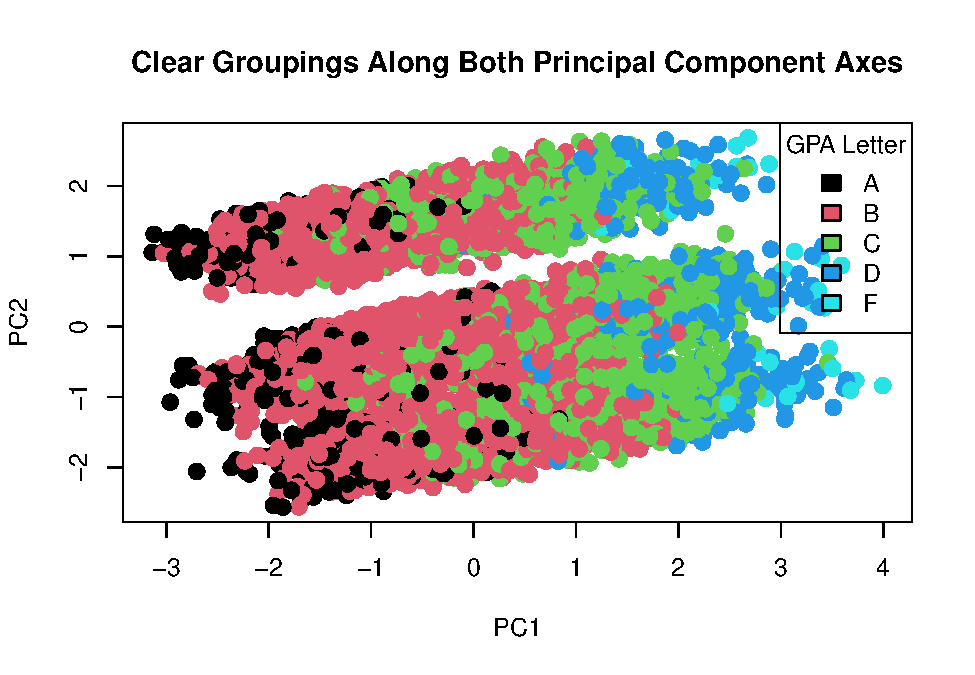
\includegraphics{ST494_FP_files/figure-latex/unnamed-chunk-10-1.pdf}

There appear to be 3 distinct groupings in the data, separable by the
second principal component. Based on the GPA letter coloring of points,
lower values of the first principal component appear to relate to higher
GPA letters and vice-versa.

\subsection{K-means Clustering: Ideal Number of
Clusters}\label{k-means-clustering-ideal-number-of-clusters}

In order to check our theory on the distinct groupings of the first two
principal components, we will employ k-means clustering. But first, we
need to determine the optimal number of clusters to effectively show
potential classes.

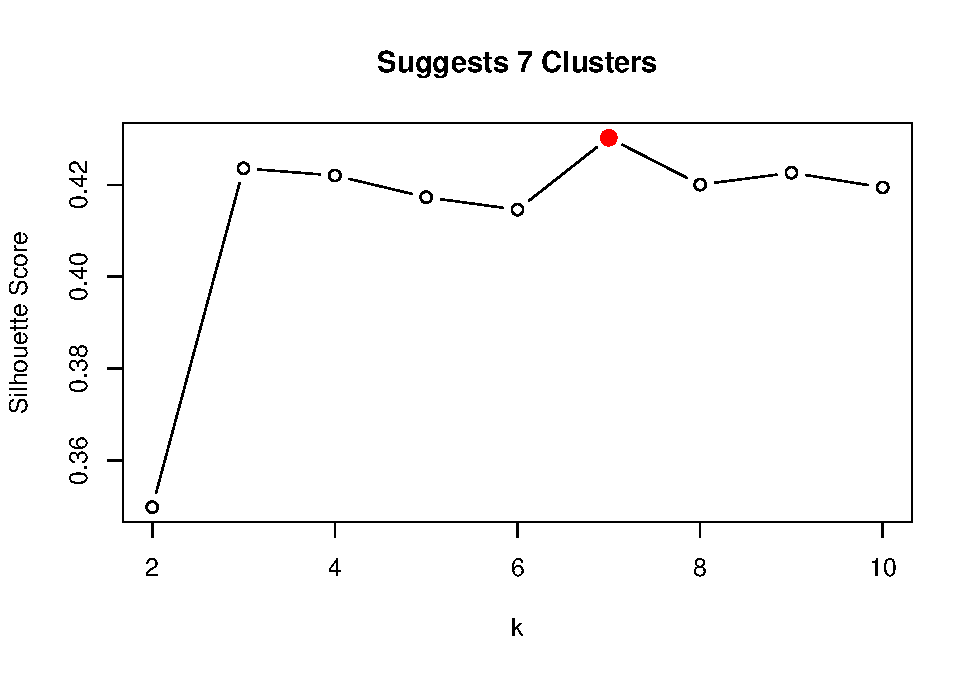
\includegraphics{ST494_FP_files/figure-latex/unnamed-chunk-11-1.pdf}

A peak in the silhouette score appears where there are 4 different
clusters, an ideal number where points are similar within a cluster and
different from other clusters.

\subsection{K-Means Clustering on First 2 Principal
Components}\label{k-means-clustering-on-first-2-principal-components}

We color the points on the same principal component graph, this time by
the cluster that they belong to.

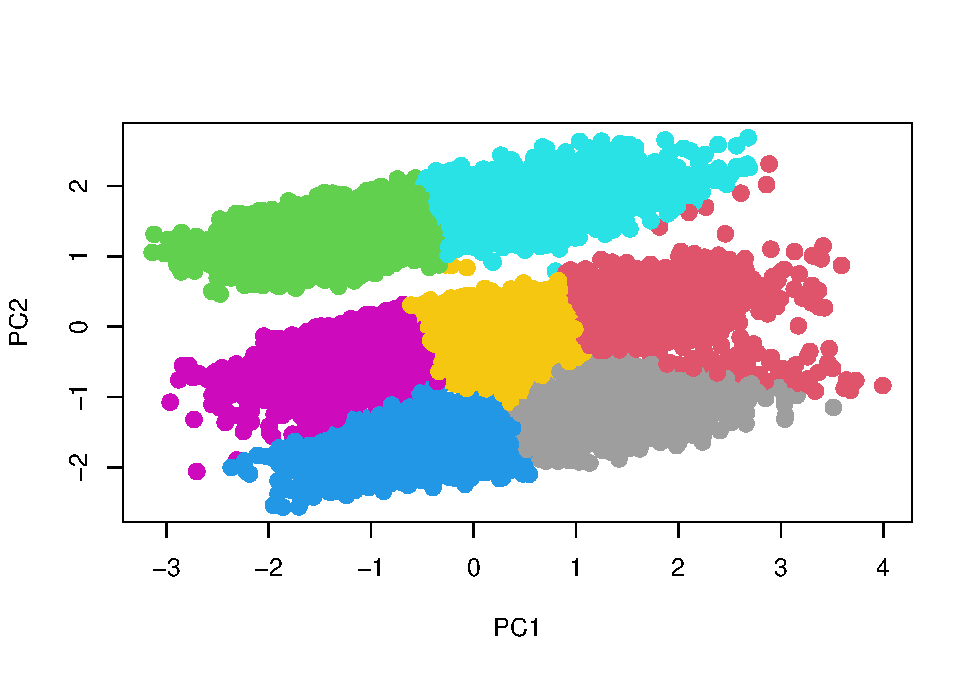
\includegraphics{ST494_FP_files/figure-latex/unnamed-chunk-12-1.pdf}

Clusters appear to be clearly separated by both principal components,
indicating that our hypothesis that the first component significantly
splits the data into groups and academic feature such as grades may
impact the second principal component appear plausible.

\subsection{Impact of Variables on the First Principle
Component}\label{impact-of-variables-on-the-first-principle-component}

We wanted to take a closer look at specific features in addition to the
overall structure of the data and principal components. So we took the
top ten largest loadings (coefficients) of the first principal
component. The goal is determine which variables are responsible for
variance within the feature set.

\begin{longtable}[]{@{}lr@{}}
\toprule\noalign{}
Variable Names & PC1 Loading \\
\midrule\noalign{}
\endhead
\bottomrule\noalign{}
\endlastfoot
is\_male & 0.5916517 \\
recent\_math\_score & -0.4443770 \\
recent\_writing\_score & -0.4309222 \\
recent\_science\_score & -0.3182190 \\
race\_ethnicityC & -0.1935130 \\
has\_subsidized\_lunch & -0.1715074 \\
parent\_educationsome high school & -0.1561814 \\
race\_ethnicityD & 0.1520213 \\
race\_ethnicityA & -0.1132013 \\
parent\_educationmaster's degree & 0.1060432 \\
\end{longtable}

Having a subsidized lunch and staying prepared appear to be the most
significant features impacting variance in the data. Although a
subsidized lunch has no obvious direct relationship to academics, it
appears that socio-economic factors may be at play in some fashion.
Taking an extra preparation course also seems to have a significant
impact in the feature space. Preparation likely has a direct
relationship with academic performance features.

\subsection{Proportion of Variance Explained
(PVE)}\label{proportion-of-variance-explained-pve}

Only the first principal component was analyzed, and other principal
components may tell very different stories about which features may be
significant. We show how much each additional principal component
contributes to the proportion of variance explained:

\begin{longtable}[]{@{}rrr@{}}
\toprule\noalign{}
Number of Principal Components & PVE & Cumulative PVE \\
\midrule\noalign{}
\endhead
\bottomrule\noalign{}
\endlastfoot
1 & 0.0922817 & 0.0922817 \\
2 & 0.0814607 & 0.1737425 \\
3 & 0.0764538 & 0.2501962 \\
4 & 0.0740256 & 0.3242218 \\
5 & 0.0733677 & 0.3975896 \\
6 & 0.0704879 & 0.4680774 \\
7 & 0.0685702 & 0.5366476 \\
8 & 0.0673422 & 0.6039899 \\
9 & 0.0631607 & 0.6671506 \\
10 & 0.0599938 & 0.7271443 \\
\end{longtable}

Additional principal components contribute significantly to higher PVE.
The first principal component does not contribute to much of the
variance explained and the second principal component does not increase
it significantly either. We interpret this to mean that there are many
notable linear combinations of features rather than a one that
significantly explains variance the feature space.

\subsection{Partial Least Squares Prediction for
GPA}\label{partial-least-squares-prediction-for-gpa}

Our analysis on the principal components is predicated on the assumption
that they having meaning in relation to evaluating academic performance.
We evaluate this by using partial least squares to predict GPA.

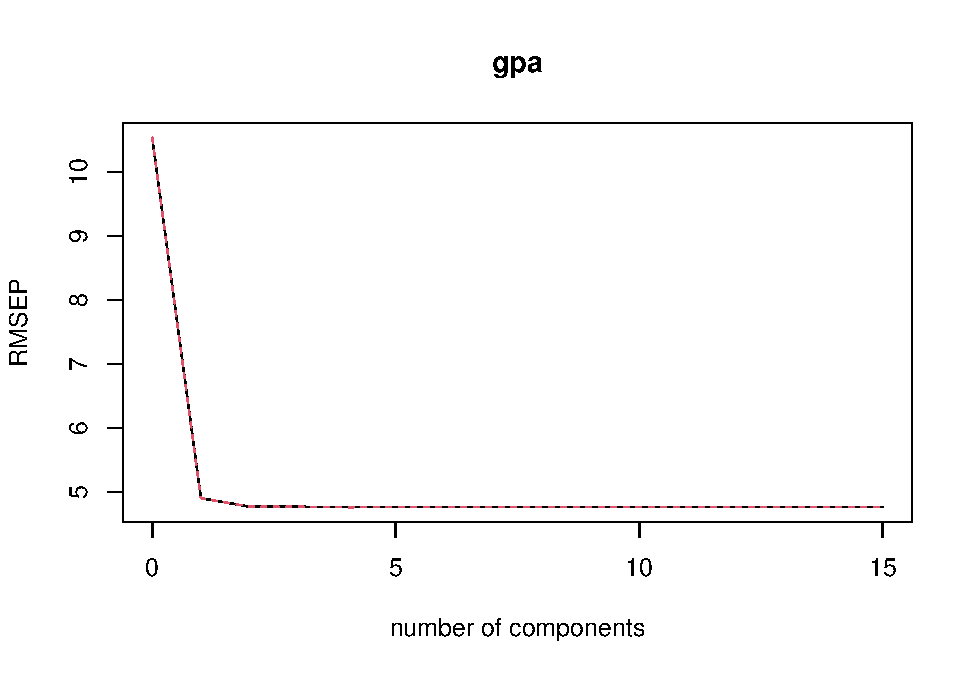
\includegraphics{ST494_FP_files/figure-latex/unnamed-chunk-15-1.pdf}

3 components appears optimal based on the PVE and plot.

\begin{longtable}[]{@{}r@{}}
\toprule\noalign{}
RMSE \\
\midrule\noalign{}
\endhead
\bottomrule\noalign{}
\endlastfoot
4.729063 \\
\end{longtable}

We will compare the error with other methods later in the analysis to
determine how effective the principal component are at predicting GPA,
our measure for academic performance.

\section{Variable Selection for Supervised
Methods}\label{variable-selection-for-supervised-methods}

Before proceeding to predict GPA with supervised linear methods, we want
to ensure that predictor variables used are relevant. It could also be
helpful to analyze which predictors contribute to academic success. This
will help to determine what factors institutions and individuals can
improve to aid in academics.

\subsection{Evaluating Criterion for Best Subset
Selection}\label{evaluating-criterion-for-best-subset-selection}

Since the dataset is not too large (\textasciitilde10000 rows), we feel
that using best-subset selection is computationally feasible and is the
optimal method for variable selection. 3 types of evaluation criterion
are employed to determine the ideal variables; AIC, BIC, and adjusted
R-squared.

\begin{verbatim}
## Reordering variables and trying again:
\end{verbatim}

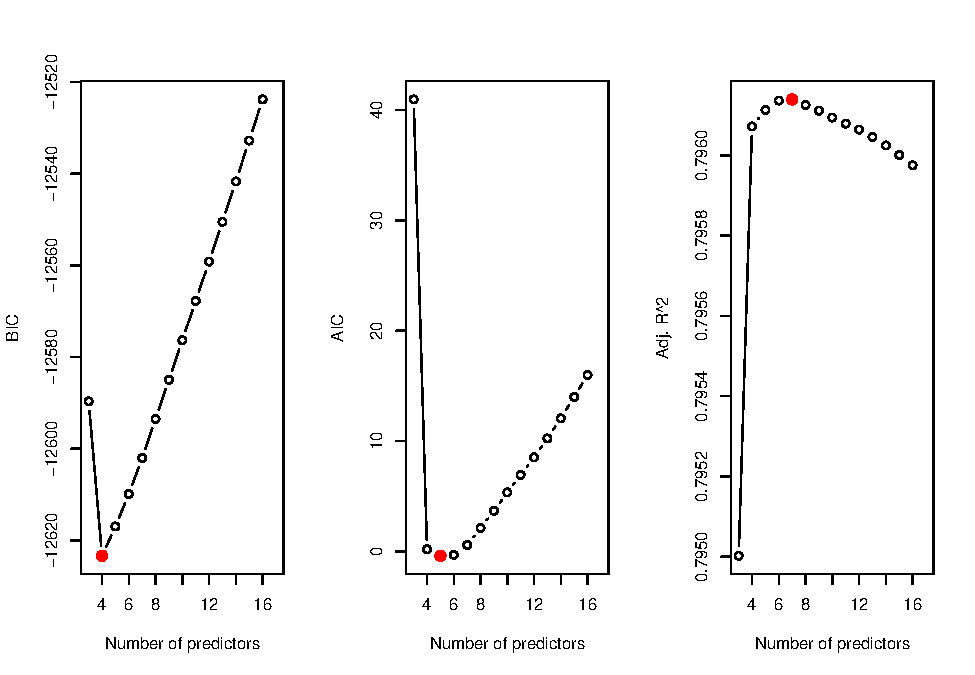
\includegraphics{ST494_FP_files/figure-latex/unnamed-chunk-17-1.pdf}

The best number of predictors appears different but fairly similar given
each criterion. BIC heavily penalizes additional variables, so it is
expected to favour a lower number of variables. AIC appears to prefer
one more variable and few more variables are favoured with
\(R^2_{adj}\).

\subsection{Ideal Number of Variables for Each
Criterion}\label{ideal-number-of-variables-for-each-criterion}

\begin{longtable}[]{@{}rrr@{}}
\toprule\noalign{}
Best\_BIC & Best\_Cp & Best\_Adjusted\_Rsq \\
\midrule\noalign{}
\endhead
\bottomrule\noalign{}
\endlastfoot
4 & 5 & 7 \\
\end{longtable}

Since BIC heavily penalizes extra predictors and adjusted \(R^2_{adj}\)
appears to be more lenient, we choose to use 6 predictors, a value in
the middle.

\subsection{Names of Ideal Predictors}\label{names-of-ideal-predictors}

The following variables contribute the most according to best subset
selection:

\begin{longtable}[]{@{}l@{}}
\toprule\noalign{}
ChosenPredictors \\
\midrule\noalign{}
\endhead
\bottomrule\noalign{}
\endlastfoot
is\_male \\
has\_prepared \\
recent\_math\_score \\
recent\_writing\_score \\
recent\_science\_score \\
parent\_educationsome high school \\
\end{longtable}

We update train and test sets to only includes these predictors.

\section{Regression for Identifying Important Predictors of Academic
Success}\label{regression-for-identifying-important-predictors-of-academic-success}

With the selected variables, we can now test how well they predict
academic performance measured in GPA. We start by training supervised
regression models to predict the GPA score.

\subsection{Choosing the Most Effective Linear
Method}\label{choosing-the-most-effective-linear-method}

The base linear regression model, as well as linear models with LASSO
and Ridge regularization are created and compared.

\begin{longtable}[]{@{}lrrr@{}}
\toprule\noalign{}
Loss Type & Unregularised Linear & LASSO & Ridge \\
\midrule\noalign{}
\endhead
\bottomrule\noalign{}
\endlastfoot
RMSE & 4.714030 & 4.714620 & 4.738995 \\
MAE & 3.874895 & 3.876661 & 3.899528 \\
\end{longtable}

Interestingly, the unregularized model outperforms LASSO and Ridge
regression. This may be because we performed regularization after
variable selection, so irrelevant predictors were already filtered out.
Additional penalties on predictors probably only interfered with making
the best predictions that minimize SSE.

\subsection{Extracting Insight And Evaluating Chosen Linear
Method}\label{extracting-insight-and-evaluating-chosen-linear-method}

Before making conclusive analysis, we want to ensure that the model is
predicting accurately on test data.

\subsubsection{Accuracy Within 10\%}\label{accuracy-within-10}

Since the linear regression model only predicts continuous values, it
wouldn't make sense to calculate accuracy directly, but we still want to
ensure that the model is accurate. We resolve this by predicting how
frequently predictions are within 10 points of the true GPA.

\begin{verbatim}
## [1] "Accuracy within 10 GPA points:  0.977409638554217"
\end{verbatim}

The vast majority of predictions are within 10 points of the true GPA,
so we feel that analysis on the impact of each attribute will be
meaningful.

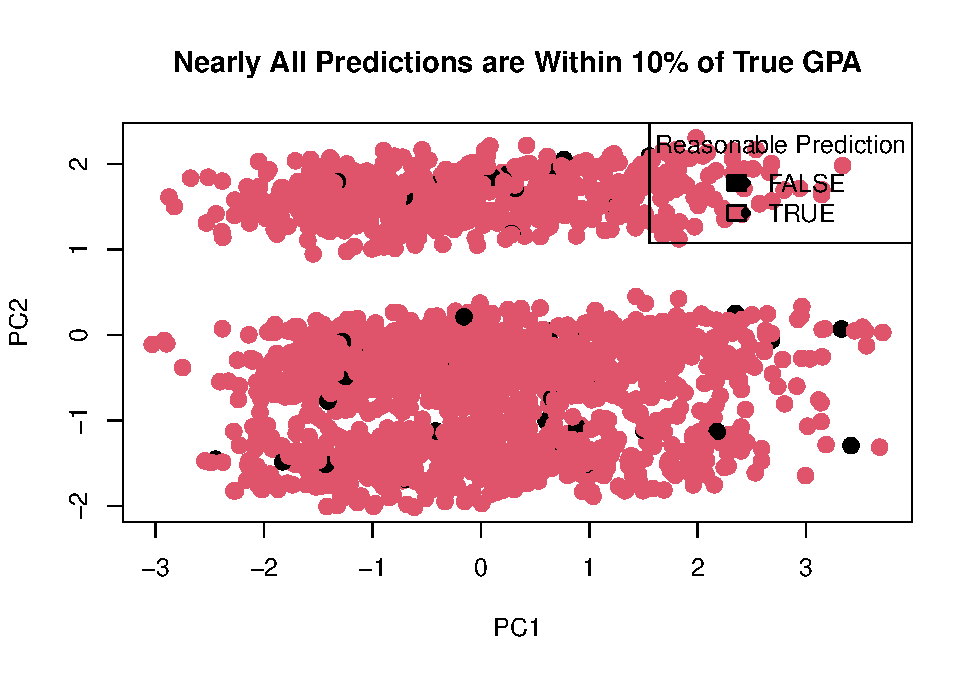
\includegraphics{ST494_FP_files/figure-latex/unnamed-chunk-23-1.pdf}

Since the model is fairly accurate at predicting GPA, we feel that
analyzing coefficients directly can provide insight into how each
predictor contributes to success.

\begin{verbatim}
##                      (Intercept)                          is_male 
##                       15.4983645                        0.7684885 
##                     has_prepared                recent_math_score 
##                        0.1515244                        0.2453538 
##             recent_writing_score             recent_science_score 
##                        0.2604180                        0.2662900 
## parent_educationsome_high_school 
##                        0.2246999
\end{verbatim}

Of the encoded variables, gender appears to be the most significant
based on the raw coefficient, followed by parent education and
preparation. These values suggest that societal factors meaningfully
impact academic success, potentially because of different educational
opportunities. Pure academic scores appear to contribute similarly to
each other. This may be because students successful in one subject tend
to be successful overall.

\subsection{Non-linear Regression: GAM}\label{non-linear-regression-gam}

Although the linear model was successful, but there remains a
possibility that prediction is more accurate with non-linear
transformations applied to variables. We employ a generalized additive
model with splines determined by cross-validation.

\subsection{Model Comparison}\label{model-comparison}

At this point we have the best supervised linear, non-linear, and
unsupervised models. By comparing each of them, we hope to obtain the
best one and to understand why it performed the best. Once the model is
understood, we will attempt to relate the model to real-world academic
performance.

\begin{longtable}[]{@{}lrrr@{}}
\toprule\noalign{}
Measurement & GAM & LinearModel & PLS \\
\midrule\noalign{}
\endhead
\bottomrule\noalign{}
\endlastfoot
RMSE & 4.7125372 & 4.7140299 & 4.7290633 \\
R2 & 0.8056238 & 0.8055003 & 0.8042583 \\
\end{longtable}

The generalized additive model performs the best in terms of RMSE.
Non-linear splines applied to predictors appear to improve the model,
indicating that GPA is not best determined by a linear combination of
features. The PLS predictions formed by the first 3 principal components
perform slightly worse, though not by a drastic margin. Reducing
dimensionality or the number of variables seems to help the model in all
methods.

Based on the results of applying regression to predict GPA, societal and
educational factors both contribute to academic success.

\section{Linear Classification for Evaluating Predictive Accuracy of GPA
Predictors}\label{linear-classification-for-evaluating-predictive-accuracy-of-gpa-predictors}

The regression models allowed us show importance within the model of
specific variables by analyzing coefficients, but we were unable to
compute easily interpretible metrics such as accuracy directly. The
purpose of our analysis is to translate our findings to the real world,
and we think that a classification perspective will provide more
interpretable results. Our goal in this section is to determine whether
a linear decision boundary can differentiate between students having a
desirable GPA.

\subsection{LDA Model}\label{lda-model}

The first classification method we attempt is linear discriminant
analysis. We train it using the same predictors determined by variable
selection.

We plot the distribution of LD1 discriminant scores to look for skew or
multimodal properties.

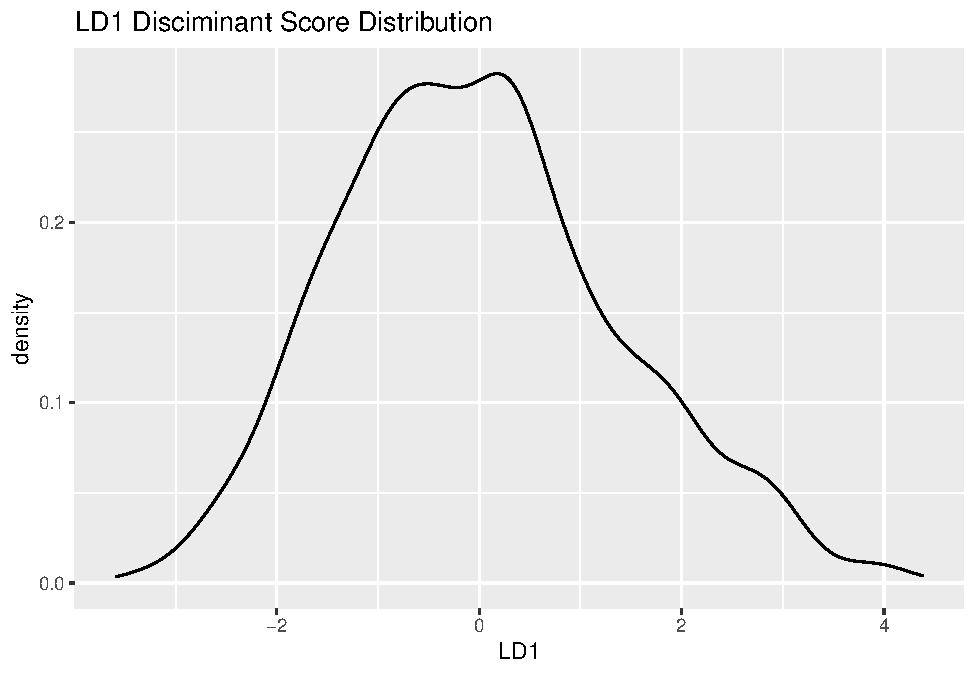
\includegraphics{ST494_FP_files/figure-latex/unnamed-chunk-29-1.pdf}

There appears to be a multimodal peak representing each class although
it is very subtle. The distribution also appears to have a slight skew
right. We interpret these properties to mean that there is a noticeable
distinction between classes and there are more extreme large
discriminant scores. This could mean that some students are strongly
predicted to have a good GPA given the predictors.

We evaluate the LDA model with a confusion matrix and related metrics.

\subsubsection{Confusion Matrix}\label{confusion-matrix}

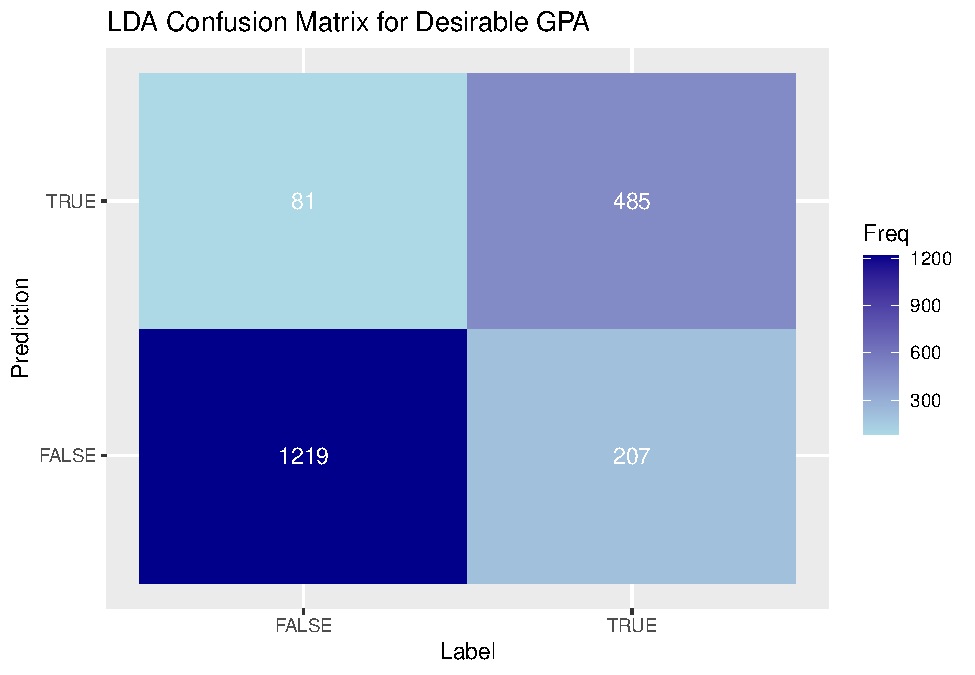
\includegraphics{ST494_FP_files/figure-latex/unnamed-chunk-30-1.pdf}

\subsubsection{Metrics}\label{metrics}

\begin{longtable}[]{@{}lr@{}}
\toprule\noalign{}
Metric & Score \\
\midrule\noalign{}
\endhead
\bottomrule\noalign{}
\endlastfoot
Accuracy & 0.8554217 \\
Sensitivity & 0.9376923 \\
Specificity & 0.7008671 \\
\end{longtable}

The LDA model seem pretty strong based on the confusion matrix and
metrics. It seems to predict the true class very well, but is not as
good at predicting true negatives. This may be due to a class imbalance.

\subsection{Logistic Model}\label{logistic-model}

\subsubsection{Confusion Matrix}\label{confusion-matrix-1}

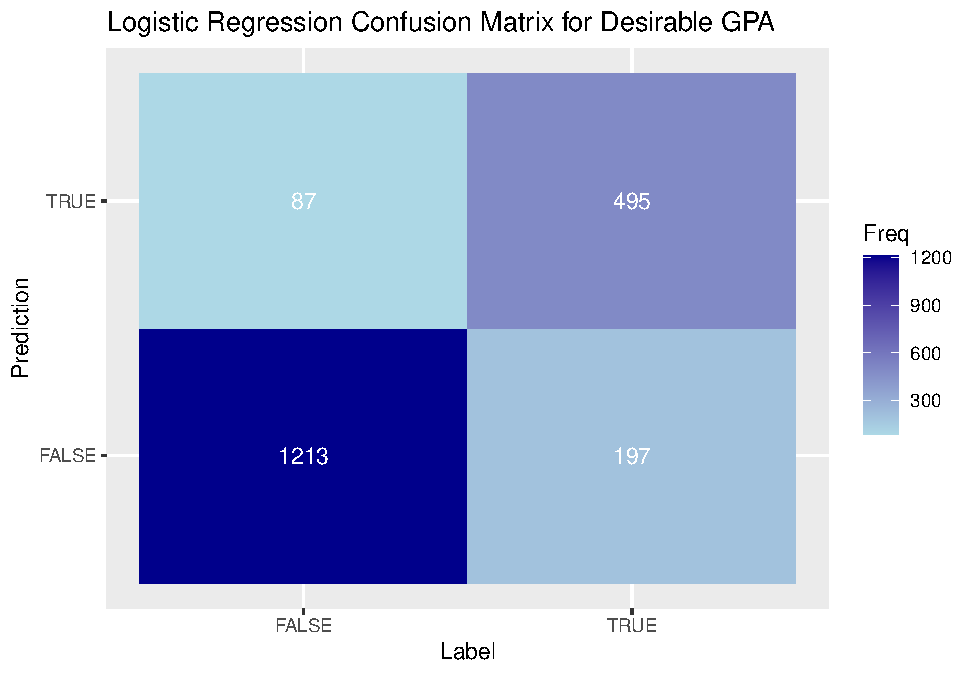
\includegraphics{ST494_FP_files/figure-latex/unnamed-chunk-34-1.pdf}

\subsubsection{Metrics}\label{metrics-1}

\begin{longtable}[]{@{}lr@{}}
\toprule\noalign{}
Metric & Score \\
\midrule\noalign{}
\endhead
\bottomrule\noalign{}
\endlastfoot
Accuracy & 0.8574297 \\
Sensitivity & 0.9330769 \\
Specificity & 0.7153179 \\
\end{longtable}

The logistic regression model appears slightly superior to the LDA model
at predicting the negative class, but results are fairly similar
overall.

\subsubsection{Plotting Logistic Regression Model
Evaluation}\label{plotting-logistic-regression-model-evaluation}

Based on the high accuracy of the linear classifiers, a linear decision
boundary can effectively differentiate between students with a good GPA
and a poor GPA. This shows that the predictors are indicative of
academic performance and if students are able to improve some of the
attributes, they are likely to be more successful in school.

\section{Classification Analysis and Visualization with Tree-Based
Methods and
SVM}\label{classification-analysis-and-visualization-with-tree-based-methods-and-svm}

We now know that the predictors can effectively distinguish between
strong and weak academic performers, but other methods may be more
accurate and provide more insight into how predictions are being made.

\subsection{Decision Tree}\label{decision-tree}

The decision tree is particularly useful for our case because it is
interpretable, and we want to show what predictive variables are causing
students to perform well in school.

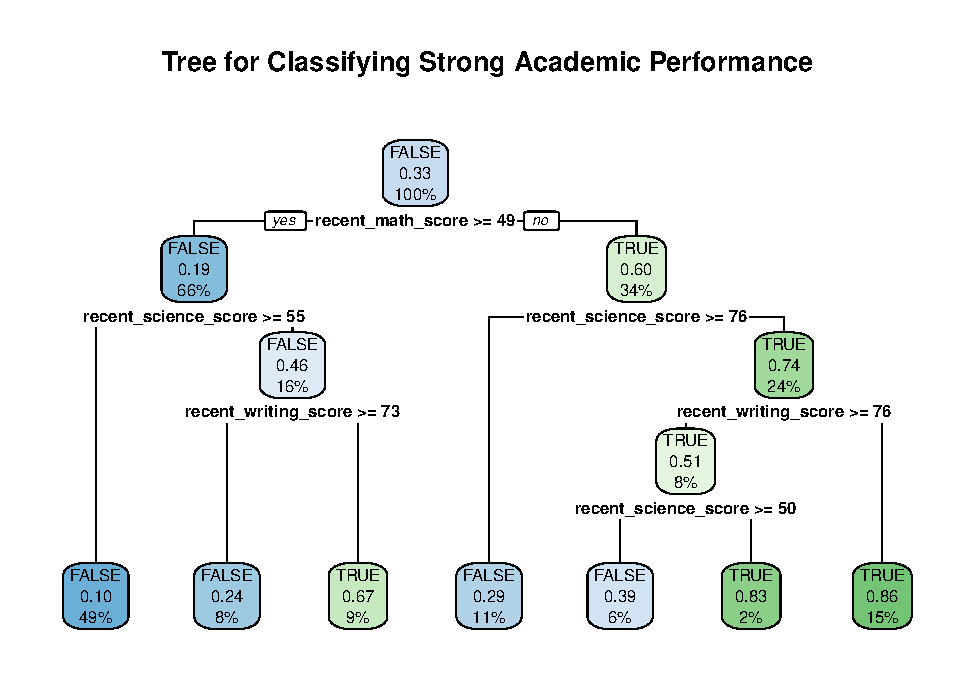
\includegraphics{ST494_FP_files/figure-latex/unnamed-chunk-38-1.pdf}

The decison tree with splits based on information gain heavily favours
academic scores for determining student performance. Among them, it
considers math the most significant split with the highest information
gain. Many areas of science rely on a strong math background, which
could explain why math score is the first split.

\subsection{Random Forest}\label{random-forest}

We follow up the decision tree by training a random forest. Since we are
attempting to extract inference rather than maximize predictive
accuracy, we do not show evaluation metrics on test data. Instead, we
plot variable importance to show which predictive variables strongly
considered by the random forest model.

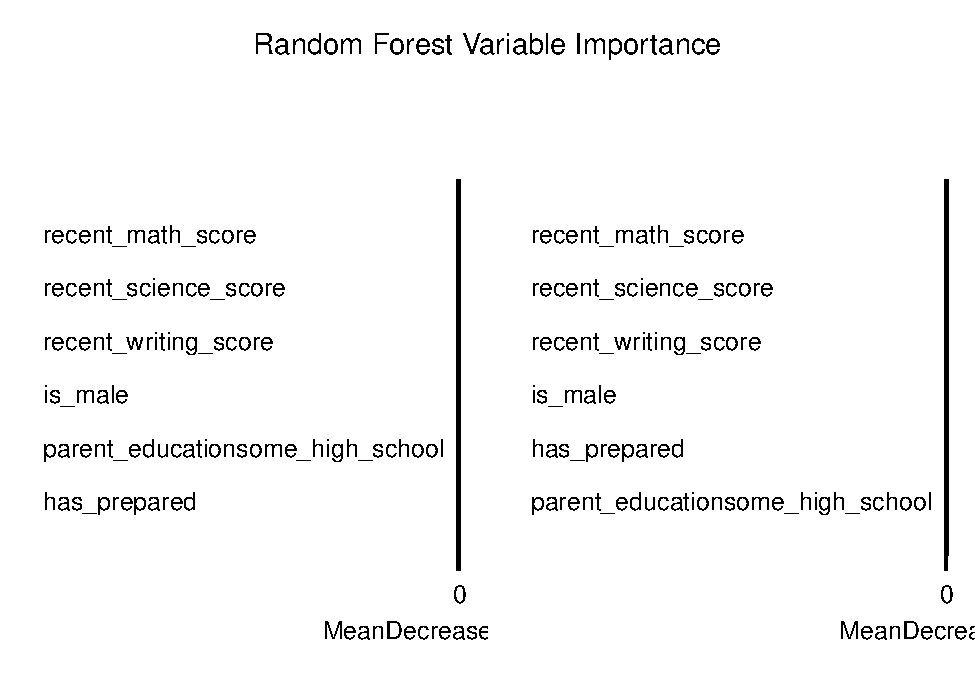
\includegraphics{ST494_FP_files/figure-latex/unnamed-chunk-40-1.pdf}

The variable importance plot strengthens the hypothesis that decision
trees and random forest heavily favour the academic predictor variables.

\subsection{SVM Kernel Analysis}\label{svm-kernel-analysis}

We apply the kernel trick to train several support vector machines in
order to analyze the ideal shape of the decision boundary.

\begin{longtable}[]{@{}lr@{}}
\toprule\noalign{}
Kernel.Type & Misclassification \\
\midrule\noalign{}
\endhead
\bottomrule\noalign{}
\endlastfoot
Linear & 0.1455823 \\
Radial & 0.1445783 \\
Quadratic & 0.3283133 \\
\end{longtable}

The support vector machine with the radial kernel performs the best,
followed closely by the linear kernel and distantly by the quadratic
kernel. Since both linear and radial kernels perform well, two seemingly
contradictory results emerge. The linear decision boundary suggests a
simpler relationship between predictor variables to classify academic
performers, while the strong performance of the SVM with the radial
kernel suggests a more complex one. In the context of academic
performance, this may mean that societal and academic predictive factors
can be used in a straightforward manner to distinguish strong academic
performers, but there are complex relationships between variables that
are better separated with a complex decision boundary.

\subsection{Deep Learning for Analyzing Specific GPA
Scores}\label{deep-learning-for-analyzing-specific-gpa-scores}

From analyzing different classification methods and kernels, we
determined that complex relationships exist between predictors of
academic success. We also previously identified that strong academic
performers can be accurately identified, but specificity tends to be far
worse than sensitivity. This leads us to think that certain GPA scores
are being misclassified consistently, while others are being classified
well. We attempt to verify the claim by creating a deep learning model
with softmax activation for multiclass classification output.

\begin{verbatim}
## [1] "A  accuracy:  20.99 %"
## [1] "B  accuracy:  76.04 %"
## [1] "C  accuracy:  80.29 %"
## [1] "D  accuracy:  61.11 %"
## [1] "F  accuracy:  0 %"
\end{verbatim}

It appears that the neural networks classifies decent grades (B) very
well. The model predicts weak albeit passing grades fairly accurately,
but performs much more poorly classifying very good or failing grades.
We think this is largely a consequence of the predictors; they are able
to identify students with performance at the extremes, either negative
or positive. This suggests that students with an A or F GPA distinguish
themselves from peers in the same circumstances as themselves. Their
individuality sets them on a unique path to achieve either great
academic success of failure.

\section{Conclusions and Future
Research}\label{conclusions-and-future-research}

\subsection{Conclusions}\label{conclusions}

\begin{itemize}
\tightlist
\item
  DOT JOT MEANT TO BE EXPANDED (just my initial ideas -LD)
\item
  previous individual subject marks = best indicator (which is best??)
\item
  impact of parent education (economic + social impact? perspectives on
  school)
\item
  lunch \textasciitilde{} income range (tends to have less access to
  resource, or luxury of time)
\end{itemize}

\subsection{Future Research}\label{future-research}

OPTIONAL????????

\begin{itemize}
\tightlist
\item
  DOT JOT MEANT TO BE EXPANDED (just my initial ideas -LD)
\item
  current emphasis on racial and economic factors + previous success
\item
  expansion of analysis possible for geographic, ie between schools with
  varying urban/rural divide,
\item
  possible opportunity to look at student mental health (IE: psycology,
  risk behaviours)
\item
  maybe even something about access to technology, a metric about
  technical capacity \textasciitilde{} assuming technical skills give
  indication for success in increasingly technical school, idk, that
  last bit is a stretch
\end{itemize}

\end{document}
